\chapter{Lecture eight: Architectural Design, Criteria and Components}

\section{Difficulties in exercises}
Final state for an object: general and in analysis and design \\
Iteration in state chart diagrams: how should it be modelled \\
Item-Descriptor pattern and the behaviour of the classes \\ 
Actor: what is and what is it not \\

\section{Why are we making these descriptions?}
\begin{itemize}
    \item A \textbf{system definition} is used in; evaluation of candidates for classes and events \textit{(chapter three)}, finding actors and use cases \textit{(chapter six)}, and finding functions \textit{(chapter seven)}.
    \item An \textbf{event table} is used in; finding candidates for structures \textit{chapter four}, and describing behavioural patterns \textit{chapter five}.
    \item \textbf{Class diagrams} is used in; describing behavioural patterns \textit{chapter five)}, and finding interface elements \textit{chapter eight)}.
    \item \textbf{Behavioural patterns} are used in; \textit{lecture nine}
    \item \textbf{Actors} are used when describing use-cases \textit{chapter six)}.
    \item \textbf{Use-cases} are used in; finding functions \textit{(chapter seven)}, and finding interface elements \textit{(chapter eight)}.
    \item \textbf{Function lists} are used in; finding interface elements \textit{(chapter eight)}.
\end{itemize}

\section{Architectural design}
\subsection{Key concepts}
So far we've talked about a \textbf{system} as a black box; a collection of components that implements modelling requirements, functions, and interfaces. Now, we'll open this box up, ignoring AD and PD, and focus on \textbf{architecture} which is; a general structure that is later developed. The architecture is a structural system view that separates system concerns. A good component architecture makes a system easier to understand. 

\subsection{Views}
There's two different views; \textbf{component architecture}, consisting of; classes, stable aspects, related components, logical level, and structure for descriptions. 

The \textbf{process architecture}, consisting of; objects, dynamic aspects, coordination of processes, physical level, and structure for execution, is the \textit{dynamic}-view, while the \textbf{component architecture} is the \textit{stable}- or \textit{static}-view. The static view will be the focus of this course.

\begin{figure}[H]
    \centering
    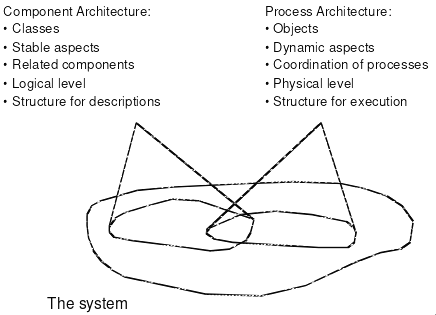
\includegraphics[width=0.5\textwidth]{figures/twoviews.png}
\end{figure}

\noindent Principles are; define and prioritise criteria, bridge criteria and technical platform, and evaluate designs early.

\subsection{Objects in Analysis and Design}
Analysis;
\begin{itemize}
    \item Phenomena outside the computer system
    \item Identity; identifies an object
    \item State; the qualities that characterise an object
    \item Behaviour; the events an object have performed or suffered
\end{itemize}

\noindent Design \textit{(and programming)}:
\begin{itemize}
    \item Phenomena inside the computer-system
    \item Identity; gets access to an object
    \item State; the values of the object's attributes and object structures
    \item Behaviour; the operations an object can perform on request and offers to other objects \textit{(methods)}
\end{itemize}

\subsection{Activities}
\textbf{Criteria, components, and processes.}
\begin{figure}[h!]
    \centering
    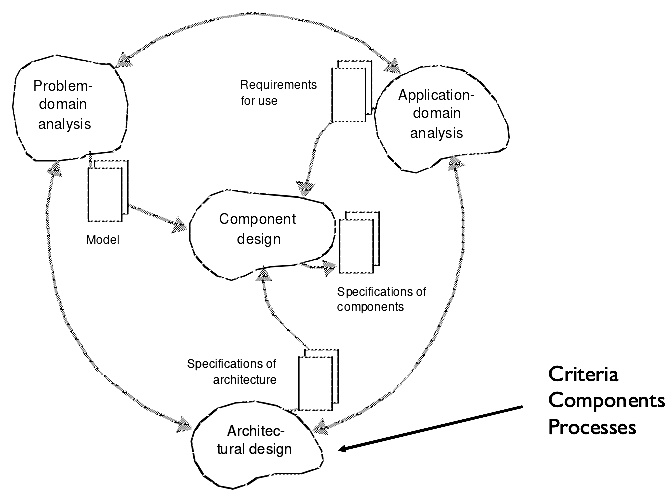
\includegraphics[width=0.7\textwidth]{figures/methodcircular.png}
\end{figure}

\subsection{Summary}

\begin{figure}[H]
    \centering
    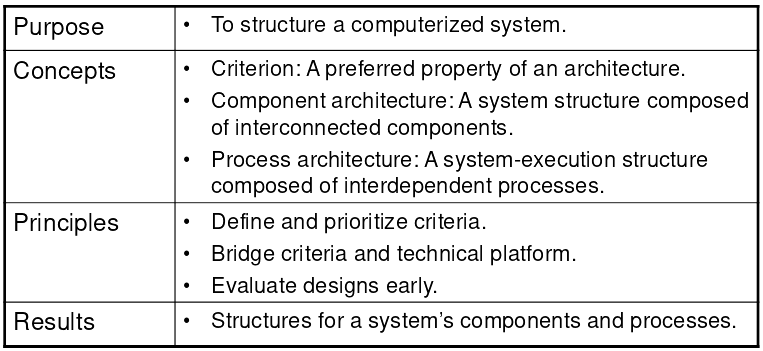
\includegraphics[width=0.65\textwidth]{figures/architecturaldesignsummary.png}
\end{figure}

\section{Criteria}
\subsection{Results}
A collection of prioritised criteria, Prioritise; emphasise which criteria is more, and less, important. Note that not all criteria can be prioritised equally important.

\begin{figure}[H]
    \centering
    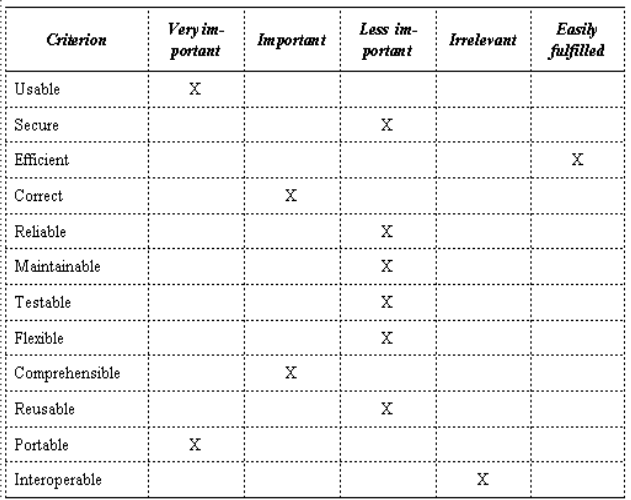
\includegraphics[scale=0.75]{figures/criteriaresult.png}
\end{figure}

\subsection{Key concepts}
General criteria, according to McCall, are:\\
\begin{minipage}[t]{\textwidth}
    \begin{minipage}[t]{.5\textwidth}
\begin{itemize}
    \item Usable
    \item Secure
    \item Efficient
    \item Correct
    \item Reliable
    \item Maintainable
    \item Testable
    \item Flexible
    \item Comprehensible
    \item Reusable
    \item Portable
    \item Interoperable
\end{itemize}
\end{minipage}%
    \begin{minipage}[t]{.5\textwidth}
Specific criteria in OOA\&D:
\begin{itemize}
    \item Usability
    \begin{itemize}
        \item The system as a whole
        \item the users' needs
        \item The technical platform
    \end{itemize}
    \item Flexibility
    \begin{itemize}
        \item Consequences of charges
        \item Modular design
    \end{itemize}
    \item Comprehensibility
    \begin{itemize}
        \item Overview
        \item Abstraction
        \item Use of patterns
    \end{itemize}
\end{itemize}
    \end{minipage}
\end{minipage}

\subsection{Activities}

\begin{figure}[H]
    \centering
    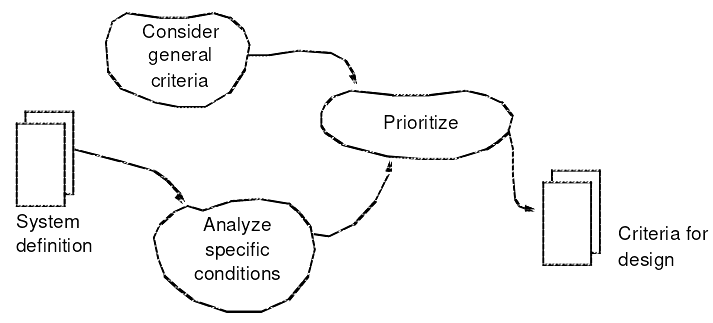
\includegraphics[width=.65\textwidth]{figures/criteriaactivities.png}
\end{figure}

\subsection{Analyse specific conditions}
Typical conditions for design of a system's architecture:
\begin{itemize}
    \item Technical:
    \begin{itemize}
        \item Technical; existing hardware, basic software, and systems
        \item Reuse of patterns and existing components
        \item Use of purchased standard components
    \end{itemize}
    \item Organisational:
    \begin{itemize}
        \item Contractual arrangements
        \item Plans for continued development
        \item Division of work between developers
    \end{itemize}
    \item Human
    \begin{itemize}
        \item Design competences
        \item Experience with similar systems
        \item Experience with technical platform
    \end{itemize}
\end{itemize}

\subsection{Example of prioritisation of a conference administration system}
Conference administration\footnote{See chapter nineteen for an explicit analysis of this}.

\begin{itemize}
    \item \textbf{Usable;} different volunteers, and many over time.
    \item \textbf{Portable;} used at each conference in different venues. 
    \item \textbf{Correct;} must fulfil the specification as the local users cannot identify and solve errors. 
    \item \textbf{Comprehensible;} must facilitate easy changes of the system. 
    \item \textbf{Efficient;} simple system for administrative tasks.
    \item \textbf{Interoperable;} stand-alone system. 
    \item \textbf{The rest;} less important because of the nature of the problem and application domains + the stable nature of these domains.
\end{itemize}

\begin{figure}[H]
    \centering
    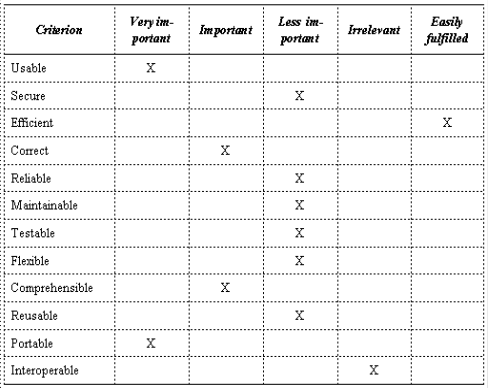
\includegraphics[scale=1]{figures/criteriaprioritize.png}
\end{figure}

\subsection{Summary}
\begin{figure}[H]
    \centering
    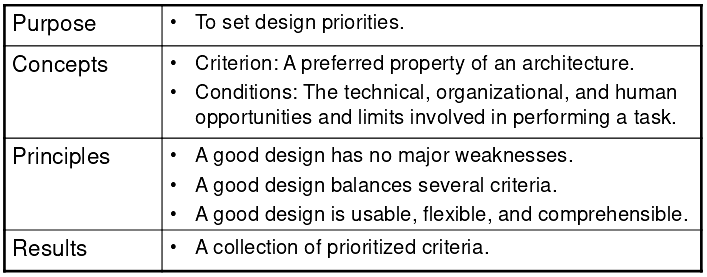
\includegraphics[width=.7\textwidth]{figures/criteriasummary.png}
\end{figure}

\begin{center}
    \textbf{A good design has no major weaknesses.}
\end{center}

\subsection{Principles}
\subsubsection{A good design has no major weaknesses}
A single flaw can be enough to invalidate a design. A good design thus strives to achieve good properties and, at the same time, avoid bad ones.

\subsubsection{A good design balances several criteria}
A good design must meet several criteria. Because these criteria can be conflicting, prioritising all criteria is essential

\subsubsection{A good design is usable, flexible, and comprehensible}
The system's usability is determined by tensions between the system's technical qualities and it's applicability to the users' work. Flexibility and comprehensibility help ease design and implementation work.

\section{The components activity}
\subsection{Results}
A structural perspective that separates concerns and responsibilities in a system. This also emphasises comprehensibility and flexibility. 
\begin{figure}[H]
    \centering
    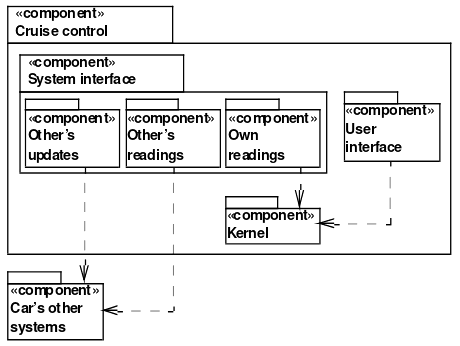
\includegraphics[width=0.5\textwidth]{figures/componentsresult.png}
\end{figure}

\subsection{Key concepts}
\subsubsection{Component}
A \textbf{component} is, at the smallest level, a class, at the largest level, a system. A component constitutes a totality and has a well-defined responsibility.

E.g. this component highlighted has the responsibility for reading the buttons and updating the display. 

\begin{figure}[H]
    \centering
    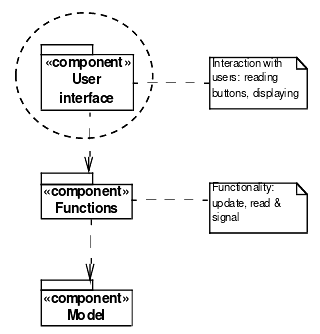
\includegraphics[width=0.35\textwidth]{figures/componentexample.png}
\end{figure}

\subsection{Activities}
From criteria, you explore architectural patterns, then both define subsystems and identify components, this results in a class diagram, after which you specify complex components and this leads to the component specification.

\begin{figure}[H]
    \centering
    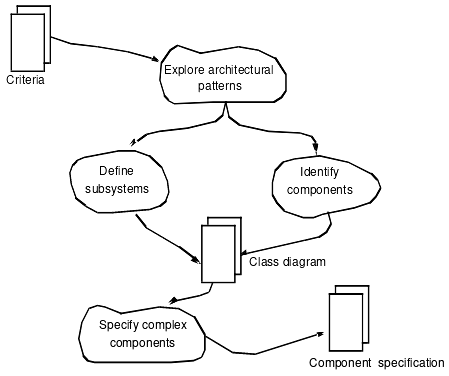
\includegraphics[width=0.5\textwidth]{figures/componentsactivities.png}
\end{figure}

\subsection{The layered architecture-pattern}
\begin{itemize}
    \item A \textbf{layer} describes a component's responsibility by the operations it provides to a layer above and those that are applied from the layer below. 
    \item A \textbf{part} has no substantial interaction with other parts of the same layer. 
    \item \textbf{Closed architecture} means that a method can only apply operations from an adjacent layer, \textbf{open architecture} can apply operations from any other layer. 
    \item\textbf{Strict architecture} means that a method can only apply operations from a layer below, \textbf{relaxed architecture} means that a method can apply operations from layer both above and below. 
\end{itemize}

\begin{figure}[H]
    \centering
    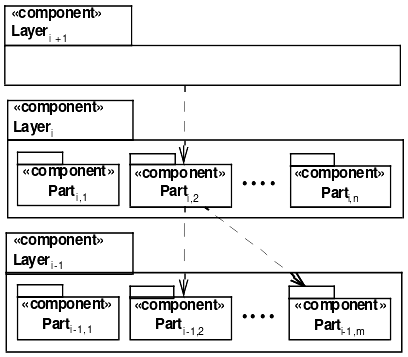
\includegraphics[width=0.4\textwidth]{figures/layeredarchitecture.png}
\end{figure}

\subsection{The generic architecture-pattern}
The \textbf{generic architecture} reflects the division of the context into problem domain and application domain. \textit{Technical platform} is an extension and encapsulation of the underlying technical platform. E.g. a Dankort-terminal.
\begin{figure}[H]
    \centering
    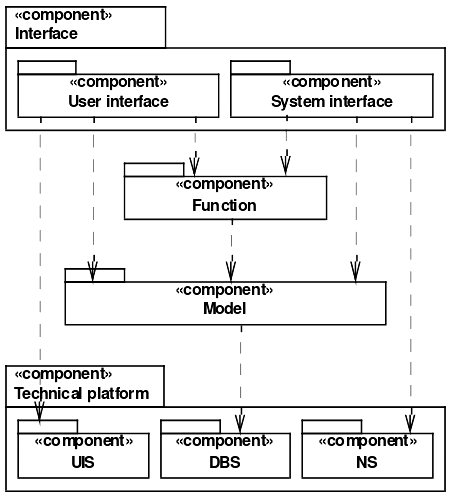
\includegraphics[width=0.45\textwidth]{figures/genericarchitecture.png}
\end{figure}

\subsection{Client-server architecture-pattern}
Originally for distribution of physical \textit{(geographically)} dispersed processors. Can also be used logically, independently of processors. One server to many clients, are the relationship. Clients are assigned to the server dynamically. The distribution can be based on various divisions between server and clients. E.g. the Dankort-operator (NETS) and the individual shops.
\begin{figure}[H]
    \centering
    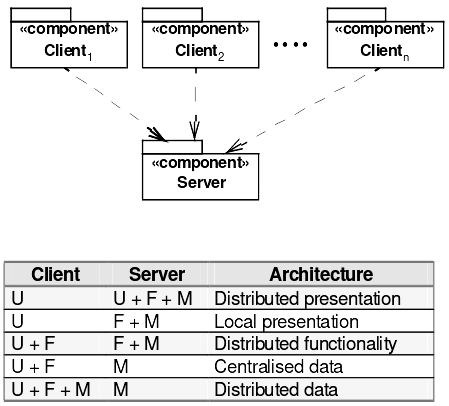
\includegraphics[width=0.4\textwidth]{figures/clientserverarchitecture.png}
\end{figure}

\subsection{Define sub-systems}
Larger system can be decomposed into several, independent sub-systems. Each sub-system has its own architecture based on the generic architecture. E.g. cruise-control and other systems of the car are related sub-systems.
\begin{figure}[H]
    \centering
    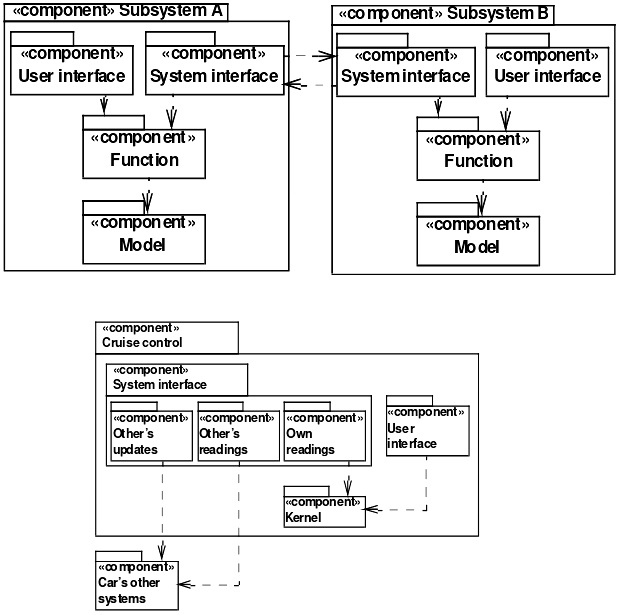
\includegraphics[width=0.6\textwidth]{figures/subsystems.png}
\end{figure}

\subsection{Specify Complex Components}
Specify the component in detail by its responsibility, dependency of other components, relation to the context. Can be done in a schema or diagram. 
\begin{figure}[H]
    \centering
    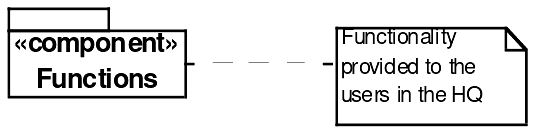
\includegraphics[width=0.35\textwidth]{figures/complexcomponents.png}
\end{figure}

\subsection{Summary}
\begin{figure}[H]
    \centering
    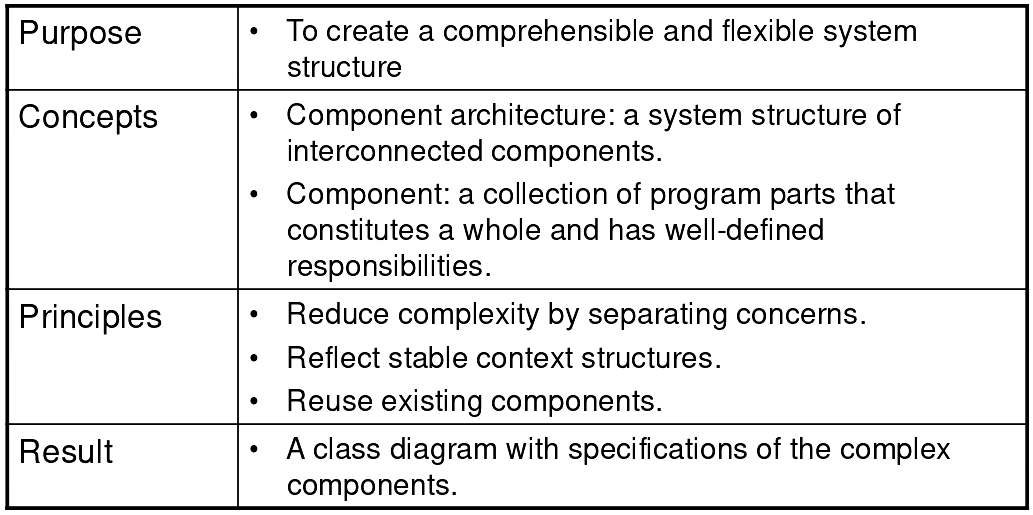
\includegraphics[width=0.5\textwidth]{figures/componentssummary.png}
\end{figure}

\subsection{Principles}
\subsubsection{Reduce complexity by separating concerns}
The components architecture should be comprehensible. Using architectural patterns makes the architecture easier to understand. Reducing complexity also eases understanding; this is achieved by separating concerns into different components.

\subsubsection{Reflect stable context structures}
The components architecture must be useful and valid in the future. To achieve this, the architecture should reflect stable aspects of the problem and application domains. At the same time, the components architecture should be flexible toward a context's unstable aspects.

\subsubsection{Reuse existing components}
Using components developed for reuse or for earlier versions of the system, or components bought off-the-shelf from a competent vendor, is an effective way to reduce the programming effort. Such components come in various forms; the right ones let you integrate previous experience and good solutions into your architecture. This contributes to a better design and less programming work.